\documentclass[12pt]{article}
\usepackage[utf8]{inputenc}
\usepackage{amsmath}
\usepackage[T1]{fontenc}

\title{ECE 3413 Lab 05\\*Time Response of First-\\*and Second-Order Systems}
\author{Leomar Dur\'an}
\date{${06}^{\text{th}}$ March 2023}

\usepackage{hyperref}

\usepackage{cancel}
\usepackage[per-mode=symbol]{siunitx}
\newcommand*\siexpr[2][]{\SI[parse-numbers=false,#1]{#2}}%
\usepackage{xfrac}
\usepackage{amssymb}
\newcommand*\transpose{\mathsf{T}}

\usepackage{mathtools}%
\DeclarePairedDelimiter\brao()%
\DeclarePairedDelimiter\brac[]%
\DeclarePairedDelimiter\braco[)%
\DeclarePairedDelimiter\Brac\{\}%
\DeclarePairedDelimiter\abs||
\DeclarePairedDelimiter\norm\lVert\rVert%
\DeclarePairedDelimiter\piecefn\{.
\DeclarePairedDelimiter\evalat.|

\usepackage{lib/nonfloatenvirons}
\usepackage{booktabs}
\newcommand\ra[1]{\renewcommand*\arraystretch{#1}}
\ra{1.25}
\usepackage{minted}

\usepackage{adjustbox}
\newcommand{\setprime}[2][1]{%
    {#2}^{%
        \raisebox{1pt}{%
            \scalebox{0.5}{%
                \itshape\sffamily\uppercase%
                \expandafter{%
                    \romannumeral#1%
                }%
            }%
        }
    }%
}%
\newcommand*\mcadj[7]%
% {#columns}{col spec}{rotation}{adjust spec}
% {before rotated text}{rotated text}{after rotated text}
{%
    \multicolumn{#1}{#2}{%
        \rlap{%
            #5\adjustbox{rotate=#3,#4}{#6}~#7%
        }%
    }%
}

\usepackage{pdfpages}
\usepackage{standalone}
\usepackage{matlab}

\usepackage[skip=\baselineskip,indent=0pt]{parskip}
\setlength\parindent{0pt}

\usepackage[shortlabels]{enumitem}

\def\hr{{\par\noindent\rule{\textwidth}{0.4pt}}}

\begin{document}

\maketitle
\newpage

\section{Introduction}

The purpose of this experiment is to apply the concept of transfer functions to a translational mechanical system.

The principles used in electrical engineering are shared with other disciplines of engineering.
We can apply these principles to help us look at everyday problems such as a translational system differently,
or we can use this familiarity to better understand the effect of a transfer function in a control system.

This lab also introduces a new type of transfer function, the state-space model which is represented by the \mintinline{matlab}{ss} class in Matlab.

\section{Procedure}

\subsection{Task 1 -- The effect of poles and natural frequency}

\begin{enumerate}[(a)]
    \item
        Given the transfer function
        \begin{equation}
            G_2\brao*s = \frac{b}{s^2 + as + b},
        \end{equation}
        
        let the damping ratio and natural frequency, respectively $\zeta, \omega_n \in \mathbb{R}$ s.t. $a = 2\zeta\omega_n$ and $b = \omega_n^2$. So
        \begin{equation}
            \piecefn*{
                \begin{matrix}
                    \omega = \sqrt{b}\rlap, \\*
                    \zeta = \dfrac{a}{2\sqrt{b}}\rlap. \\*
                \end{matrix}
            }\rlap{$\qquad\brao*{b > 0}$}
        \end{equation}

        Furthermore
        \begin{equation}
            \zeta\omega_n = \frac{a}2,
        \end{equation}
        and
        \begin{equation}
            \sqrt{1 - \zeta^2} = \sqrt{1 - \brao*{\sfrac{a}{\brao*{2\sqrt{b}}}}^2} = \frac{1}{2\sqrt{b}} \sqrt{4b - a^2}.%
            \hskip1em\brao*{\abs*{a} \leq 2\sqrt{b}}
        \end{equation}
        
        We find that the peak time
        \begin{equation}
            T_p = \frac\pi{\omega_n \sqrt{1 - \zeta^2}} = \frac\pi{\brao*{\sqrt{b}}\brao*{ \frac{1}{2\sqrt{b}}\sqrt{4b - a^2}}} = \frac{2\pi}{\sqrt{4b - a^2}}.
        \end{equation}

        We find that the overshoot rate
        \begin{equation}
            \begin{array}{*2{@{}r}@{}l@{}}
                \% OS
                &{}:={}& \exp\brao*{\dfrac{-\zeta\pi}{\sqrt{1 - \zeta^2}}} \SI{100}\percent
            \\*[1.3em]
                &{}={}& \exp\brao*{-\zeta\omega_n\brao*{\dfrac{\pi}{\omega_n\sqrt{1 - \zeta^2}}}} \SI{100}\percent
            \\*
                &{}={}& \exp\brao*{-\brao*{\zeta\omega_n}^{\vphantom{1}}T_p} \SI{100}\percent
            \\*
                &{}={}& \exp\brao*{-\brao*{\tfrac{a}2}^{\vphantom{1}}T_p} \SI{100}\percent
            \\*
                & {}={} & \exp\brao*{\dfrac{-aT_p}{2}} \SI{100}\percent\rlap.
            \\*
            \end{array}
        \end{equation}

        We find that the settling time
        \begin{equation}
            T_s \approx \frac4{\zeta\omega_n} = \frac4{\brao*{\sfrac{a}2}} = \frac8a.
        \end{equation}

        To find rise time, we must first find the step response in the time domain with parameters substituted.

        \subsubsection{Step response}
        We have
        \[
            G_2\brao*s = \frac{b}{s^2 + as + b},
        \]

        Well
        \begin{equation}
            C\brao*s = R\brao*s G_2\brao*s = \frac1s \frac{b}{s^2 + as + b}.
        \end{equation}

        So the second order factor of the denominator
        \begin{equation}\label{eq:sum of squares}
            \begin{aligned}
                s^2 + as + b
                &{} = \brao*{s^2 + 2\brao*{\frac{a}2}s + \brao*{\frac{a}2}^2} + \brao*{b - \brao*{\frac{a}2}^2}
            \\*
                &{} = \brao*{s + \frac{a}2}^2 + \brao*{\sqrt{b - \brao*{\frac{a}2}^2}}^2
                \rlap{
                    $\hskip0.5em\brao*{\abs*{a} \leq 2\sqrt{b}}$
                }
            \\*
                &{}= \brao*{s + \hat{a}}^2 + \omega^2.
            \\*
            \end{aligned}
        \end{equation}

        Thus, for $G_2\brao*s$, we have
        \begin{equation}
            \piecefn*{
                \begin{array}{@{}l@{}}
                    \displaystyle
                    \hat{a} = \frac{a}2, \\*
                    \omega = \sqrt{b - \hat{a}^2}. \\*
                \end{array}
            }
        \end{equation}

        Thus, we find coefficients $A,B,C$ s.t.
        \begin{equation}
            b = A\brao{s^2 + as + b} + B\brao{s^2 + \hat{a}s} + C\omega s.
        \end{equation}

        Asume $s = 0$. Then
        \begin{equation}
            s = 0: b = A\brao{\cancel{\brao*0^2} + \cancel{a\brao*0} + b} + B\brao*{\cancel{\brao*0^2} + \cancel{\hat{a}\brao*0}} + \cancel{C\omega \brao*0}.
        \end{equation}
        So $b = Ab$. Thus $A = 1$. Thus
        \begin{equation}
            b = \brao{s^2 + as + b} + B\brao{s^2 + \hat{a}s} + C\omega s.
        \end{equation}
        For quadratic terms, we have $0s^2 = s^2 + Bs^2$. So $B = -1$. Thus
        \begin{equation}
            b = \brao{s^2 + as + b} - \brao{s^2 + \hat{a}s} + C\omega s.
        \end{equation}
        Finally, for linear terms, we have $0s = as - \hat{a}s + C\omega s$. Thus
        \begin{equation}
            C = \frac{\hat{a} - a}\omega
            = \frac{\displaystyle\brao*{\frac{a}2} - a}\omega
            = \frac{-a}{2\omega},\ 
            % = \frac{\displaystyle\brao*{\frac{a}2} - a}{\displaystyle\sqrt{b - \brao*{\frac{a}2}^2} } = \frac{-a}{\sqrt{4b - a^2}}.
            \omega = \sqrt{b - \brao*{\frac{a}2}^2} \not= 0.
        \end{equation}

        Then by the inverse Laplace transform, in the time domain, we have step response
        \begin{equation}
            \begin{aligned}
                c\brao*t = \brao*{1 + \brao*{-\cos\brao{\omega t} - \frac{a}{2\omega} \sin\brao{\omega t} }{e^{-\brao*{\sfrac{a}2}t}}}u\brao*t,\ 
                \omega = \sqrt{b - \brao*{\frac{a}2}^2}.
            \end{aligned}
        \end{equation}

        After this step, we cannot solve the general case for $t$. So we must first evaluate $c\brao*t$ at some values for $a, \omega$.

        \subsubsection{Evaluations}
        Let's evaluate at $a = 4, b = 25$. Well
        \begin{equation}
            \piecefn*{
                \begin{array}{@{}l@{}}
                    b = \brao*{25} > 0,
                \\*
                    \abs{a} = \abs{4} = 4 < 10 = 2\sqrt{\brao{25}} = 2\sqrt{b},
                \\*
                    \omega = \sqrt{\brao{25} - \brao*{\frac{\brao*4}2}^2} = \sqrt{21} \not= 0
                \\*
                \end{array}
            }
        \end{equation}
        The peak time
        \begin{equation}
            T_p = \frac{2\pi}{\sqrt{4\brao{25} - \brao4^2}} = \siexpr{0.6\overline956}\second.
        \end{equation}
        The overshoot rate
        \begin{equation}
                \% OS
                ={} \exp\brao*{\frac{-\brao4\brao{\SI{0.6856}\second}}2} \SI{100}\percent = \siexpr{2\overline5.3802}\percent.
        \end{equation}
        The setting time
        \begin{equation}
            T_s \approx \frac84 = \SI2\second.
        \end{equation}

        For the rise time, in the time domain, the step response
        \begin{equation}
            \begin{aligned}
                c\brao*t = \brao*{1 + \brao*{-\cos\brao{\omega t} - \frac{a}{2\omega} \sin\brao{\omega t} }{e^{-\brao*{\sfrac{a}2}t}}}u\brao*t.
            \end{aligned}
        \end{equation}

        Assuming that $a > 0$, then the final value is s.t.
        \begin{equation}
            c\brao*t
            \xrightarrow{t\to+\infty} \brao*{1 + \brao*{-\cos\brao{\omega t} - \frac{a}{2\omega} \sin\brao{\omega t} }\cancel{\brao*{e^{-\brao*{\sfrac{a}2}t}}}^0} \cancel{u\brao*t}^1 = 1 = c_f.
        \end{equation}

        Thus, the $\SI{90}\percent$ and $\SI{10}\percent$ values are $.9c_f = 0.9$ and $.1c_f = 0.1$ respectively.

        Well $a = 4,\ \omega = \sqrt{21} \not= 0$.
        Using these known values, we can use the script in Appendix subsection~\ref{sap:solving for .9cf and .1cf}, we find the times corresponding to these values
        \begin{equation}
            \piecefn*{
                \begin{array}{@{}l@{}}
                    t_{.9} = \SI{0.388761}\second, \\*
                    t_{.1} = \SI{0.096063}\second. \\*
                \end{array}
            }
        \end{equation}
        Thus, rise time $T_r = t_{.9} - t_{.1} = \SI{0.388761}\second - \SI{0.096063}\second = \SI{0.292698}\second$.

        \subsubsection{Plotting the poles and zeroes}
        Although the poles and zeros may be plotted with the built-in Matlab function \mintinline{matlab}{pzmap}, which accepts a transfer function or system and plots its zeroes and poles,
        I have written the Matlab script in Appendix subsection~\ref{sap:pzplot} showing how it works with results in Fig.~\ref{fig:pzplot_1a}

    \item
        \subsubsection{Effect of the pole's imaginary part}
        \paragraph{On transfer function parameters}
        In \eqref{eq:sum of squares}, we found that the denominator of transfer function $G_2\brao*s$ is $s^2 + as + b = \brao{s + \hat{a}}^2 + \omega^2$.

        Thus the poles $s$ s.t.
        \begin{equation}
            \begin{aligned}
                0 &{}= \brao*{s + \hat{a}}^2 + \omega^2
            \\*
                  &{}= \brao*{s + \hat{a}}^2 - \brao*{j\omega}^2
            \\*
                  &{}= \brao*{s + \brao*{\hat{a} - j\omega}}\brao*{s + \brao*{\hat{a} + j\omega}},
            \\*
            \end{aligned}
        \end{equation}
        that is
        % \begin{equation}
            % \begin{aligned}
                $s_{1,2} = -\hat{a} \pm j\omega$.
            % \\*
                    % &{}= -\frac{a}2 \pm j\sqrt{b - \brao*{\frac{a}2}^2}.
            % \end{aligned}
        % \end{equation}

        Assuming that $\omega\in\mathbb{R}$, then $s_{1,2} = \mathfrak{Re}\brao*s \pm j\mathfrak{Im}\brao*s$,
        the real part of $s_{1,2}$,
        \begin{equation}
            \mathfrak{Re}\brao*s := \frac{s_1 + s_2}2 = -\hat{a} = -\frac{a}2,
        \end{equation}
        and the imaginary part
        \begin{equation}
            \mathfrak{Im}\brao*s := \abs*{\frac{s_1 - s_2}{2j}} = j\omega = \sqrt{b - \hat{a}^2}.
        \end{equation}

        Thus, we have parameters $a,b$ s.t. $a = -2 \mathfrak{Re}\brao*s$, and
        \begin{equation}
            \begin{aligned}
                b &{}= \mathfrak{Im}^2\brao*s + \hat{a}^2
            \\*
                & {}= \mathfrak{Im}^2\brao*s + \brao*{-\mathfrak{Re}\brao*s}^2
            \\*
                & {}= \brao*{\mathfrak{Re}^2 + \mathfrak{Im}^2}\brao*s.
            \\*
            \end{aligned}
        \end{equation}

        Let $m,n \in \mathbf{R}$, and let $\setprime{s}_{1,2} = m\mathfrak{Re}\brao*s + jn\mathfrak{Im}\brao*s$, s.t.
        \begin{equation}
            \piecefn*{
                \begin{matrix}
                    \mathfrak{Re}\brao*{\setprime{s}} = m\mathfrak{Re}\brao*s,
                \\*
                    \mathfrak{Im}\brao*{\setprime{s}} = n\mathfrak{Im}\brao*s.
                \\*
                \end{matrix}
            }
        \end{equation}

        Thus the new parameters,
        \begin{equation}
            \piecefn*{
                \begin{array}{@{}l@{}}\displaystyle
                      \setprime{a}
                    = -2\mathfrak{Re}\brao*{\setprime{s}}
                    = -2m\mathfrak{Re}\brao*s
                    \rlap,
                \\*
                      \setprime{b}
                    = \brao*{\mathfrak{Re}^2 + \mathfrak{Im}^2}\brao*{\setprime{s}}
                    = \brao*{\tilde{m}\mathfrak{Re}^2 + \tilde{n}\mathfrak{Im}^2}\brao*s
                    \rlap.
                \\*
                \end{array}
            }
        \end{equation}

        Further, in comparison with the original parameters,
        the new parameters
        \begin{equation}
            \piecefn*{
                \begin{array}{@{}l@{}}\displaystyle
                      \setprime{a}
                    = -2m\brao*{-\frac{a}2}
                    = -ma
                    \rlap,
                \\*
                      \setprime{b}
                    = \brao*{m\brao*{-\dfrac{a}2}^2 + n\brao*{\sqrt{b - \brao*{-\dfrac{a}2}^2}}^2}
                    = \brao*{m - n}\brao*{\dfrac{a}2}^2 + nb
                    \rlap.
                \\*
                \end{array}
            }
        \end{equation}

        \paragraph{On transfer function parameters}
\end{enumerate}



\section{Results}

\subsection{Poles and zeroes of $G_2$}

\begin{figure}
    \centering
    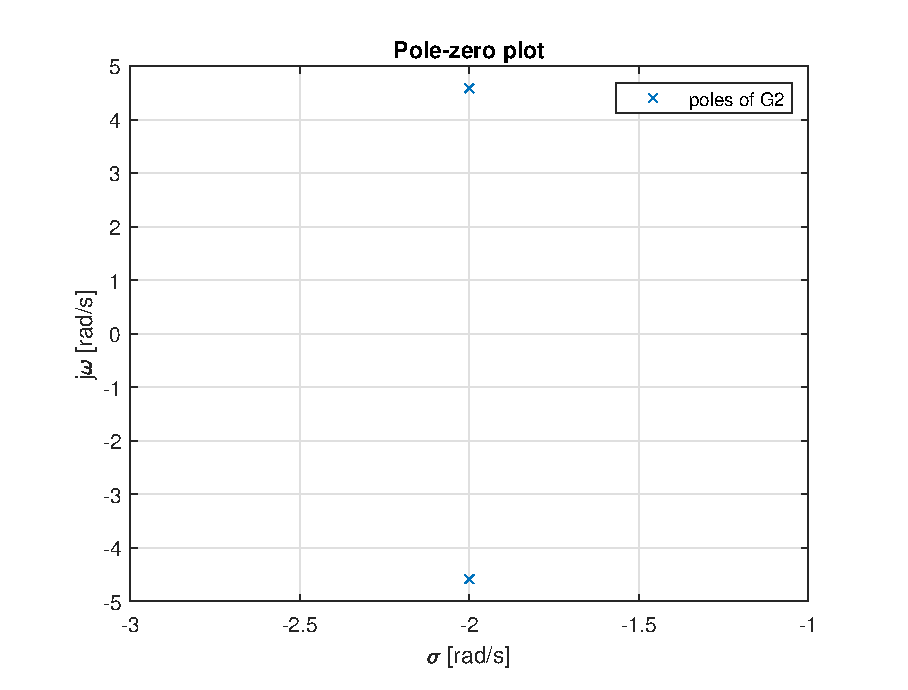
\includegraphics[width=\linewidth]{img/part01a_pzplot.eps}
    \caption{A custom pole-zero plot of the transfer function $G_2$ in part~01(a).}
    \label{fig:pzplot_1a}
\end{figure}



\section{Discussion}

After finding the state-space representation,
this experiment becomes very straightforward.
However, that is the difficult part.

What I remembered to help me finish it is that springs act on displacement into the moving mass and viscous dampers aft on velocity away from the moving mass.
After this, the sum of all forces must equal the acceleration of the mass.
Then setting up the matrix of coefficients is not difficult although I may not have been able to think of coming up with the variables myself.
It's a really clever way of solving this problem.

This experiment shows application not only in electrical engineering, but also mechanical and civil engineering of the concept of a control system.
It's interesting to imagine how many of the concepts that we have learned in electrical engineering may be applied to other engineering disciplines or may have even come from methods in other engineering disciplines.

Often times, it seems that less intuitive techniques may make a problem much easier to solve simply by changing the domain or a basis.
This is the principle behind using the Laplace transform to handle transfer functions more easily.

\newpage
\appendix
\section{Appendix}

\subsection{Part 1a -- Rise time, Matlab script}\label{sap:solving for .9cf and .1cf}
\inputminted{matlab}{src/part01a_rise_time.m}

\subsection{Part 1a -- Pole-zero plot, Matlab Live Script}\label{sap:pzplot}
\inputminted{matlab}{src/part01a_pzplot_mlx.m}

\end{document}
